\documentclass{article}
\usepackage{graphicx}
\usepackage{float}
\usepackage{titlesec}
\usepackage{datetime}
\usepackage{geometry}
\usepackage{placeins}
\usepackage{minted}
\usepackage{xcolor}
\usepackage{listings}
\usepackage{caption}
\usepackage[document]{ragged2e}
\usepackage[hidelinks]{hyperref}
\usepackage{enumitem}
\geometry{
 a4paper,
 left=25mm,
 top=25mm,
 }
\captionsetup{hypcap=false} 
\newdateformat{daymonthyear}{\THEDAY .\THEMONTH .\THEYEAR}
\title{
  \centering
  
\includegraphics[width=\textwidth]{images/logo_PWr_kolor_poziom.png}\\
  \fontsize{28pt}{30pt}\selectfont Sprawozdanie 7\\
  \fontsize{14pt}{30pt}\selectfont Ćwiczenie 7.WebGL}
\author{Krzysztof Zalewa}
\date{\daymonthyear\today}
\renewcommand*\contentsname{Spis treści}
\renewcommand{\figurename}{Rysunek}
\renewcommand{\listingscaption}{Fragment kodu}
\begin{document}
    \maketitle
    \pagebreak
    \tableofcontents
    \FloatBarrier
    \section{Wstęp teoretyczny}
        \subsection{WebGL}
            \raggedright
            WebGL jest Api pozwalającym na renderowanie 2D i 3D w obiekcie canvas z html (W przeglądarkach które 
            na to pozwalają). Programy urzywające WebGL składają się z kodu głównego napisanego w JavaScript i 
            kodu shaderów napisanego w GLSL. Kod ten jest następnie wykonywany przez kartę graficzną urządzenia.
            \begin{figure}[ht]
                \centering
                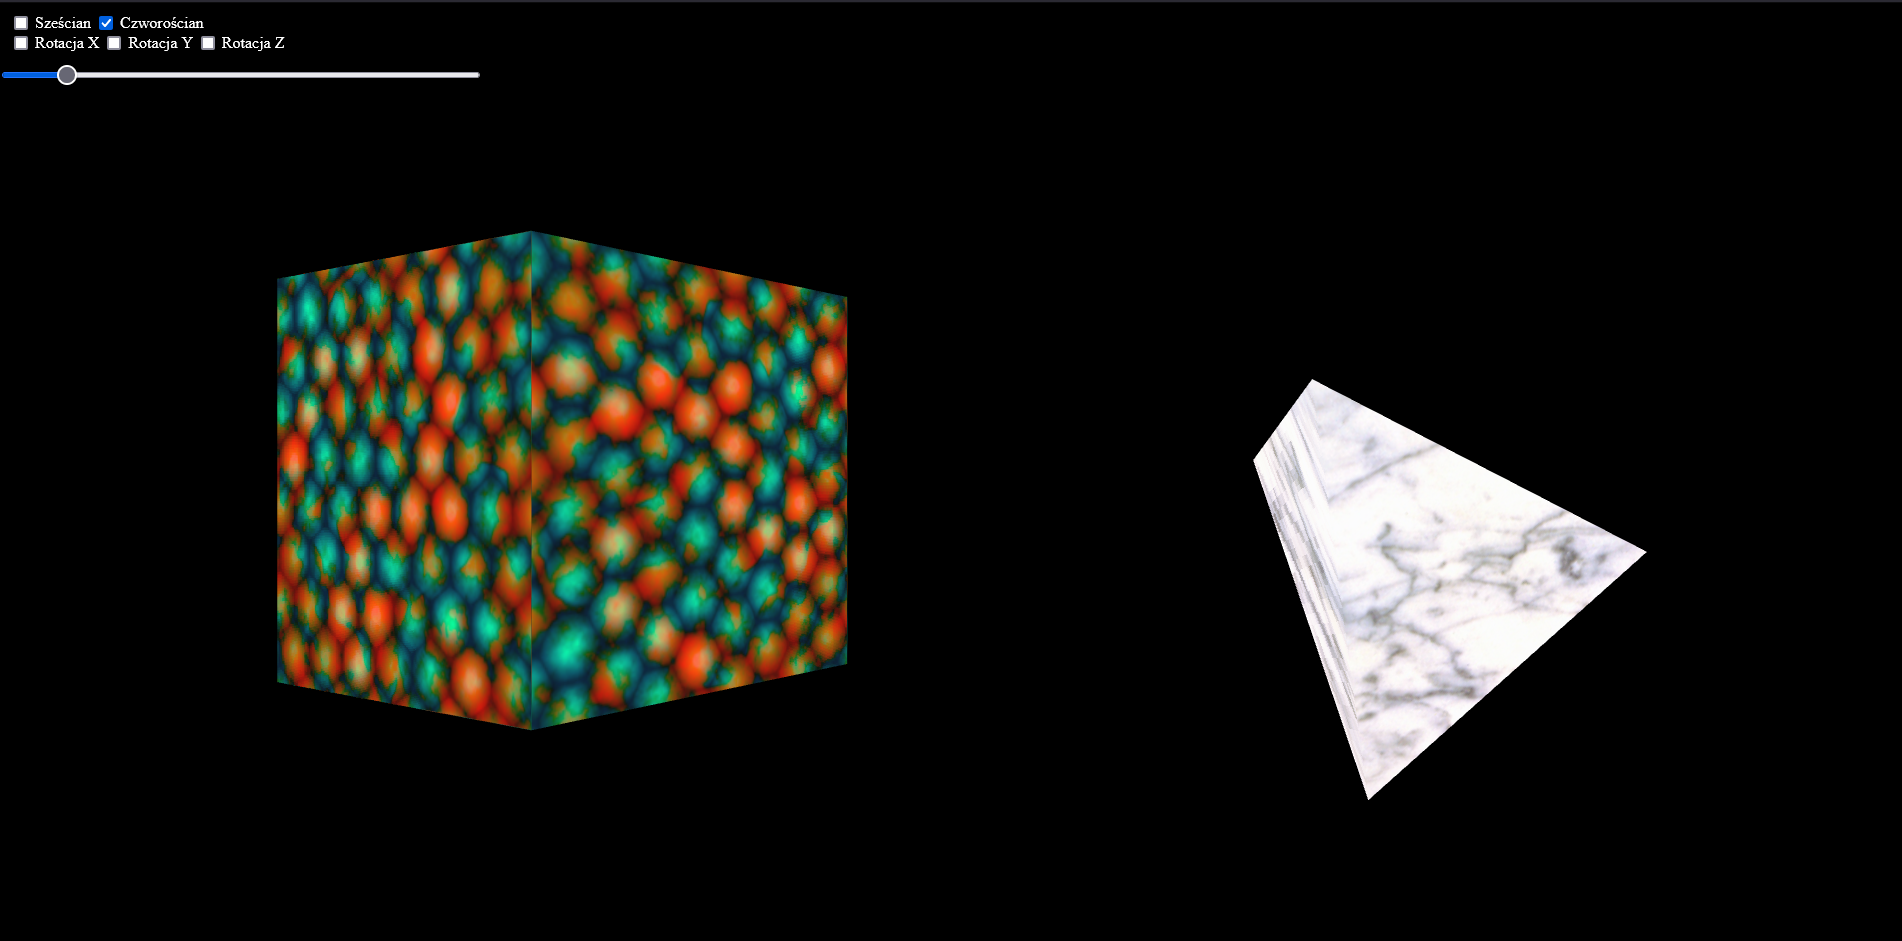
\includegraphics[width=\textwidth]{images/WebGl.png}
                \caption{Przykład programu z wykorzystaniem WebGL}
                \label{fig:webgl}
            \end{figure}
            \FloatBarrier
        \subsection{GLSL}
            Język programownia potoku graficznego (ang. OpenGL Shading Language). Język ten jest używany w nowszych 
            wersjach OpenGL zamiast niektórych funkcji wbudowanych ponieważ pozwala on na znacznie większą elastyczność
            modelu programownia potoku graficznego. W moim programie zaimplementowanłem dwa shadery:
            \begin{enumerate}
                \item \textbf{Shader wierzchołków} - Za każdym razem gdy kształt jest renderowany dla każdego wierzchołka
                uruchamiany jest shader wierzchołków. Jego zadaniem jest transformacja oryginalnych kordynatów na kordynaty 
                używane przez WebGL (W zakresie -1.0 do 1.0). Shader ten może mieć wiele atrybutów które min. pozwalają 
                określić kordynaty tekstury. Na koniec przetransofrmowana pozycja przekazywana jest do WebGL przez specjalną
                zmienną \textbf{gl\_Position}.
                \begin{frame}
                    \scriptsize
                    \begin{minted}[
                        style=vs,
                        breaklines,
                        breakanywhere, 
                        linenos, 
                        tabsize=4 
                    ]{js}
                        const vsSource = `
                        attribute vec4 aVertexPosition;
                        attribute vec2 aTextureCoord;
                        uniform mat4 uModelViewMatrix;
                        uniform mat4 uProjectionMatrix;
                        varying highp vec2 vTextureCoord;
                        void main(void) {
                            gl_Position = uProjectionMatrix * uModelViewMatrix * aVertexPosition;
                            vTextureCoord = aTextureCoord;
                        }
                        `;
                    \end{minted}
                    \vspace{1em}
                    \captionof{listing}{Przykładowy shader wierzchołków}
                    \label{lst:vsSource}
                \end{frame}
                \item \textbf{Shader fragmetów} - Za każdym gdy shader wierzchołków wykona swoje zadanie i narysuje wierzchołki
                zaczynają być rysowane pojedyńcze piksele. Shader fragmetów jest wywoływany dla każdego piksela. Jego zadaniem
                jest wybranie koloru danego piskela na podstawie tekseli(piksel w teksturze). Następnie kolor jest przekazywany
                do WebGL przez specjalną zmienną \textbf{gl\_FragColor}. Następnie odpowiedni kolor jest rysowany w miejscu piksela.
                \begin{frame}
                    \scriptsize
                    \begin{minted}[
                        style=vs,
                        breaklines,
                        breakanywhere, 
                        linenos, 
                        tabsize=4 
                    ]{js}
                        const fsSource = `
                        varying highp vec2 vTextureCoord;
                        uniform sampler2D uSampler;
                        void main(void) {
                            gl_FragColor = texture2D(uSampler, vTextureCoord);
                        }
                        `;
                    \end{minted}
                    \vspace{1em}
                    \captionof{listing}{Przykładowy shader fragmentów}
                    \label{lst:fsSource}
                \end{frame}
            \end{enumerate}
    \section{Zadanie laboratoryjne}
        \raggedright
        \subsection{Treść zadania}
            W ramach zadania laboratoryjnego należało napisać program kożystający z WebGL.
            Program ten miał wyświetlić dwa obiekty sześcia z brakującą ścianką i czworościan.
            Powinna być możliwość obrotu obiektów, wyboru który obiekt obracamy oraz zwiększenie
            lub zmniejszenie prędkości obrotu.
        \subsection{Opis działania programu}
            Program rysuje obiekty zgodnie z treścią zadania. W prawym górnym rogu znajdują się 
            przyciski które pozwalają na kontrolę obracania. Poniżej przycisków znajduje się suwak
            który pozwala na przyspieszenie lub zwolnienie animacji.
        \subsection{Kod programu}
            \begin{frame}
                \scriptsize
                \inputminted[
                    style={vs},
                    breaklines,
                    breakanywhere, 
                    linenos, 
                    tabsize=4 
                ]{html}{indexTex.html}
                \vspace{1em}
                \captionof{listing}{Fragment kodu z programu}
                \label{lst:html}
            \end{frame}
            \begin{frame}
                \scriptsize
                \inputminted[
                    style={vs},
                    breaklines,
                    breakanywhere, 
                    linenos, 
                    tabsize=4 
                ]{js}{./js/Lab7.js}
                \vspace{1em}
                \captionof{listing}{Fragment kodu z programu}
                \label{lst:main}
            \end{frame}
            \begin{frame}
                \scriptsize
                \inputminted[
                    style={vs},
                    breaklines,
                    breakanywhere, 
                    linenos, 
                    tabsize=4 
                ]{js}{./js/init-buffers.js}
                \vspace{1em}
                \captionof{listing}{Fragment kodu z programu}
                \label{lst:init}
            \end{frame}
            \begin{frame}
                \scriptsize
                \inputminted[
                    style={vs},
                    breaklines,
                    breakanywhere, 
                    linenos, 
                    tabsize=4 
                ]{js}{./js/draw-scene.js}
                \vspace{1em}
                \captionof{listing}{Fragment kodu z programu}
                \label{lst:draw}
            \end{frame}
    \section{Źródła}
        \begin{enumerate}[label=\arabic*.]
            \item \url{https://pl.wikipedia.org/wiki/OpenGL_Shading_Language}
            \item \url{https://www.khronos.org/opengl/wiki/Core_Language_(GLSL)}
            \item \url{https://developer.mozilla.org/en-US/docs/Web/API/WebGL_API/Tutorial/Getting_started_with_WebGL}
            \item \url{https://developer.mozilla.org/en-US/docs/Web/API/WebGL_API/Tutorial/Adding_2D_content_to_a_WebGL_context}
            \item \url{https://developer.mozilla.org/en-US/docs/Web/API/WebGL_API/Tutorial/Animating_objects_with_WebGL}
            \item \url{https://developer.mozilla.org/en-US/docs/Web/API/WebGL_API/Tutorial/Creating_3D_objects_using_WebGL}
            \item \url{https://developer.mozilla.org/en-US/docs/Web/API/WebGL_API/Tutorial/Using_textures_in_WebGL}
        \end{enumerate}
\end{document}